\chapter{Grundlagen}
\markboth{Grundlagen}{}
\label{ch:Grundlagen}

In diesem Kapitel wird zuerst auf das Projekt WBS Alarm eingegangen und die Anforderungen an die Erfassung der Transaktionen ausführlich beschrieben. Hier soll erläutert werden, welche Gedankengänge hinter den Anforderungen stecken. 

Danach werden zwei Fallstudien vorgestellt, die sich mit dem Kostenwachstum der Entwicklung und Wartung mit fortschreitenden Releases, also Veröffentlichungen eines Softwareprodukts, beschäftigt haben. Hier werden die wichtigsten Erkenntnisse aus den Fallstudien zusammengefasst.

Im Folgenden wird in Kapitel~\ref{sec:Softwarearchitektur} auf einzelne Details einer sauberen Softwarearchitektur eingegangen. In den Kapiteln~\ref{sec:Designprinzipien} und~\ref{sec:Komponentenprinzipien} werden einige Prinzipien für die Entwicklung leicht wart"= und erweiterbarer Software vorgestellt. 

\section{WBS Alarm}
\label{sec:wbs}

WBS Alarm ist ein Warenbestandssystem, das für die freiwillige Feuerwehr in Eschenstruth im Laufe des Studiums Sozialinformatik entwickelt wurde. Die Software entstand aus dem Bedürfnis, einen Überblick über den aktuellen Bestand an Kleidung und ihrer Verteilung zu schaffen. Dies wurde zuvor auf externen Datenträgern wie Tafeln, Zetteln und als Microsoft Excel Tabelle auf einem USB Stick verteilt. Diese Variante war auf Dauer von den Mitgliedern der Feuerwehr nicht mehr zu handhaben, da die Informationen mit der Zeit auseinandergeflossen sind und der Überblick schwand. Daher sollte eine Software entwickelt werden, die diesen Missstand aufhebt. Über einen Zeitraum von zwei Jahren wurde das Projekt abgeschlossen und ist mittlerweile in einem produktiven Zustand. 

Im Wesentlichen wird in WBS Alarm ein Träger der freiwilligen Feuerwehr verwaltet. Im Beispiel von Eschenstruth wäre dies die Gemeinde Helsa. Unter dem Träger werden die Anwender, Zielorte und Kleidungsstücke verwaltet. Bei der Anlage eines Trägers werden vier Zielorte angelegt: Wareneingang, Lager, Wäscherei und Aussonderung. Der Wareneingang hat als Sonderstellung keine verwaltbaren Bestände, da alle Einkäufe darüber gebucht werden. Der Wareneingang selbst steht aber nicht als Zielort für Buchungen zur Verfügung. Es steht den Administrator*innen die Option offen, in WBS Alarm eigene Wareneingänge zu erstellen. Somit könnten Lieferanten abgebildet werden. Die Wäscherei ist aus der Anforderungsanalyse mit der freiwilligen Feuerwehr entstanden.

Die Transaktionserfassung ist der zentrale Punkt der Software und stellt als komplexesten Teil den Kern des Systems dar. Die Anforderungen an eine Transaktion werden wie folgt definiert: 

\begin{itemize}
\item Ein Anwender kann nur für seinen eigenen Träger eine Transaktion erfassen.
\item Eine Transaktion hat immer genau einen Ursprungsort und einen Zielort.
\item Der Ursprungsort und der Zielort müssen unterschiedlich sein.
\item Der Urspungsort und der Zielort gehören zum Träger des Anwenders.
\item Eine Transaktion umfasst mindestens eine Position. 
\item Eine Position besteht aus einem Kleidungsstück und dessen Anzahl.
\item Ein Kleidungsstück darf nur in einer Position pro Transaktion vermerkt sein.
\item Das verbuchte Kleidungsstück ist im Ursprungsort in der gewünschten Anzahl vorhanden --- dies gilt sofern es sich beim Ursprungsort nicht um den Wareneingang handelt, über den neue Kleidungsstücke aufgenommen werden. 
\item An den Wareneingang darf nicht gebucht werden.
\item Die Orte müssen für die Erfassung gesperrt sein, \dah ein Ort, dessen Bestand durch einen administrativen Anwender initial erfasst worden ist, muss für weitere Änderungen gesperrt werden. Somit wird eine Manipulation der Bestandswerte vermieden. Wenn bei einer Inventur Missstände festgestellt werden, muss eine Korrektur über die Buchungsschnittstelle erfolgen.
\end{itemize}

Diese Anforderungen muss eine Transaktion erfüllen, um in WBS Alarm verbucht zu werden.


\section{Kostenwachstum je Release}
\label{sec:Kostenwachstum}

In einer Fallstudie hat \citeauth{martin2018} das Kostenwachstum für jedes erbrachte Release untersucht. Dabei hat er aus einem untersuchten Unternehmen, das anonym bleiben wollte, den Lebenszyklus eines marktführenden Softwareprodukts analysiert. Der Umfang des Entwicklungsteams hat über acht Releases signifikant zugenommen (\refAbb{fig:staff_rel}), die Anzahl der Zeilen an Quellcode hat sich ab einem gewissen Punkt aber nicht mehr stark vermehrt (\refAbb{fig:kloc_rel}). Die Produktivität des Entwicklerteams (\refAbb{fig:prod_rel}) fiel schon ab dem vierten Release mit jedem weiteren Release immer weiter gegen Null. Für das Entwicklerteam ist das frustrierend, da alle Bemühungen das Produkt zu erweitern, den Aufwand und die Anstrengungen für zukünftige Produktversionen vermehrt \citep[vgl.][5\psqq]{martin2018}. 

Bei der Analyse der Probleme ist \citeauth{martin2018} auf zwei wesentliche Faktoren gestoßen. Zum einen musste das Produkt schnell auf den Markt gebracht werden. Den Quellcode strukturieren und aufräumen könne aus Sicht der Projektleitungen danach erledigt werden und wurde entsprechend verschoben. Diese Vorgehensweise wurde aber weiterhin durchgeführt, da der Marktdruck nicht nachgelassen hat. Somit wurde die Wartung und Pflege des vorhandenen Quellcodes immer weiter aufgeschoben. Der andere Faktor war die Annahme, dass unordentlicher Code auf kurze Sicht einen Geschwindigkeitsvorteil bringt und alles andere langfristig nur aufhält \citep[vgl.][10]{martin2018}.

Der beste Weg die Lebensdauer von Softwareprodukten gewinnbringend zu erhöhen ist laut \citeauth{martin2018}, der Qualität der eigenen Softwarearchitektur mehr Bedeutung beizumessen und ernster zu nehmen \citep[vgl.][12]{martin2018}.


\begin{figure}
  \centering
  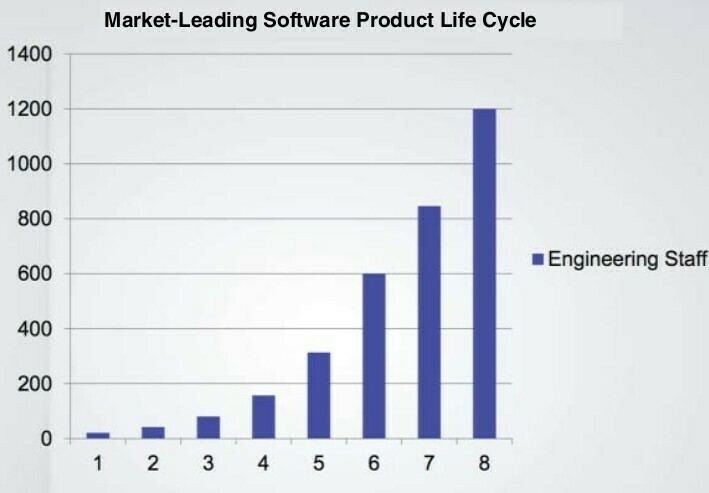
\includegraphics[width=.6\textwidth]{res/staff_releases.jpg}
   \caption{Personalwachstum im Entwicklungsbereich mit jedem Release \citep[][5]{martin2018}.}
   \label{fig:staff_rel}
\end{figure}


\begin{figure}
  \centering
  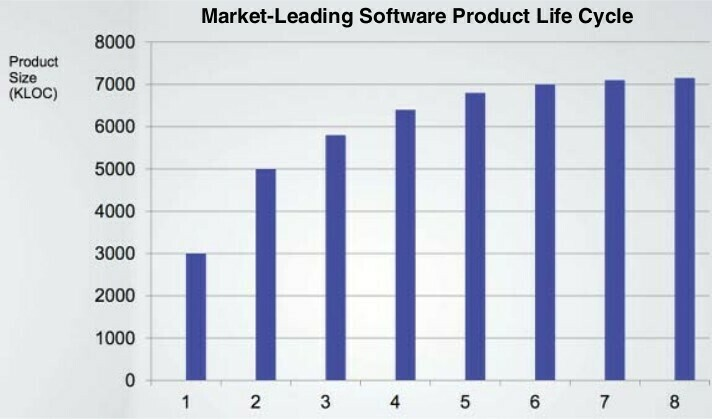
\includegraphics[width=.6\textwidth]{res/kloc_releases.jpg}
   \caption{Anzahl Zeilen an Quellcode mit jedem Release \citep[][6]{martin2018}.}
   \label{fig:kloc_rel}
\end{figure}


\begin{figure}
  \centering
  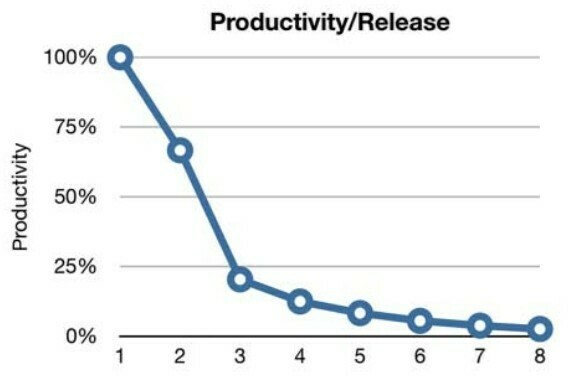
\includegraphics[width=.6\textwidth]{res/productivity_releases.jpg}
   \caption{Produktivität des Entwicklungsteams mit jedem Release \citep[][8]{martin2018}.}
   \label{fig:prod_rel}
\end{figure}


In einer weiteren Fallstudie setzt \citeauth{Ogheneovo2014} die Komplexität und die Instandhaltungs"= und Evolutionskosten von Software in Verbindung. Da Software sich über die Zeit weiter entwickelt (\textit{Evolution}), wird sie gleichzeitig auch komplexer, wenn nicht der Quellcode restrukturiert wird um die Komplexität zu verringern. Dies kann \zb als Ergebnis einer Instandhaltungsmaßnahme sein. Unter Evolution einer Software kann die Erweiterung von Funktionen verstanden werden, die einen weiteren Nutzerkreis ansprechen soll. Auch der Einsatz von neuen Technologien, um neuen Funktionen gerecht zu werden, fallen als Evolutionskosten an \citep[vgl.][3]{Ogheneovo2014}.

%\textquote[{\cite[][3]{Ogheneovo2014}}]{Software maintenance and evolution of systems was first proposed by Lehman in 1969 [11]. Lehman notes that systems continue to evolve over time. As a result, they become more complex unless some action such as code refactoring is adopted to reduce the complexity that may arise as a result of maintenance. [...] 
%The software value can be enhanced by expanding the customer base, meeting additional requirements, thus making the software more easier to use, more efficient, more reliable, and employing new technology to cater for the new features that may be introduced to these technologies. Software evolution plays an important role in software maintenance process. Most development effort and expenditure is allocated to the evolution and update of existing versions of software. Software is ceaselessly changed—maintained, evolved and updated—more often than it is written, and changing software is extremely costly.}.

In die Instandhaltungsphase fallen 60 bis 70\% der Aufwände. Damit umfasst sie den größten Teil der Entwicklung und auch einen Großteil der kompletten Lebenszykluskosten \citep[vgl.][3]{Ogheneovo2014}.

%\textquote[{\cite[][3]{Ogheneovo2014}}]{Barry et al. [14] notes that about 60 to 70\% effort is expended on maintenance phase of software development life cycle. It therefore suffix to say that software maintenance activities span a system’s productive life cycle and consume a major part of the total life cycle costs of the system. The software maintenance process can last for years or even decades after development process [15]. Therefore, there is need for effective planning in order to address the scope of software maintenance, the tailoring of the post delivery/deployment, the designation of who will pro- vide maintenance, and an estimation of the life-cycle costs. Software maintenance takes more effort than all the other phases of software life cycle.}.

Ein Faktor, der die Instandhaltungskosten verringern kann, ist die Modularisierung der Software. Hiermit werden Teile der Software in einzelne Module aufgeteilt und wieder neu miteinander verbunden. Durch die logische Aufteilung des Softwaredesigns kann die Komplexität verringert und die einzelnen Module wartbarer gemacht werden. In der Entwicklung spielt das Konzept der Modularisierung eine wichtige Rolle. \textit{Microsoft} hat mehr als drei Jahre gebraucht um \textit{Windows Vista} letztendlich zu veröffentlichen. Hier waren die Module logisch so groß aufgebaut, dass die Programmkomplexität anstieg. Mit jedem Patch und jeder Verbesserung wurde es schwieriger neue Funktionalitäten einzuführen. Deshalb mussten Untermodule geschaffen werden, welche die Komplexität verringerten. Durch die fehlende Strukturierung und Modularisierung des Programmcodes verzögerte sich die Markteinführung von \textit{Windows Vista} \citep[vgl.][8\psq]{Ogheneovo2014}.

%\textbf{Factors Affecting Software Maintenance Costs}
%\textquote[{\cite[][8\psq]{Ogheneovo2014}}]{Modularity: Modularity is the degree to which system’s components may be separated or recombined. In modular programming, modularity refers to the compartmentalization and inter-relation of the parts of a software system. It is the logical partitioning of software design that allows complex software to be manageable for the purpose of implementation and maintenance. This logic may be based on related functions, implementation considerations, data links etc. Baldwin and Clark [41] in their theory note that modular architectures add value to system designs by creating options to improve the system by substituting or experimenting on individual modules.
%The concept of modularity is very important in software development and maintenance. According to [42], it took Microsoft more than three years of delay before they finally released Windows Vista. This was attributed to the presence of large modules which made the software to increase program complexity. Therefore, for large modules to be meaningful and useful in a program, they must be broken down into smaller modules called sub-modules. Guth [43] opined that the delay was attributed to complexity resulting from the system’s lack of modularity. According to him, with each patch and enhancements, it became harder to strap new features into the software, since new code could affect everything else in unpredictable ways. This is why Walter [44] concluded that Microsoft Windows Vista is a 60-m- ines-of-code mess of spaghetti. This is because the code lacks pattern, is unstructured, and is not well modularized. Thus Microsoft suffered from unanticipated depen- dencies, modularity decay, and delays in bringing software to market. As seen from above, it is clear that there is no firm or organization that has been able to solve the problem of software complexity. According to Fried, even a firm with deep expertise in software development, like Microsoft, can still suffer from a complexity disaster resulting from a system’s lack of modularity.}.

Hier wurde auch festgestellt, dass mit jeder weiteren Version von Windows das Entwicklerteam immer weiter anwuchs. Von den Anwender*innen wurden mehr Funktionen gefordert, weswegen der Druck gewachsen ist die Deadline zu treffen. Aber je mehr Entwickler*innen an dem Code arbeiteten desto mehr Fehler entstanden \citep[vgl.][12]{Ogheneovo2014}.

%% --- MAYBE aber Übergang?--- %%
%\textquote[{\cite[][12]{Ogheneovo2014}}]{The table also shows that in each release of Windows version, the size of the development team is on the increase. This is because as more functionalities are needed by users, so there is pressure on the software  development team to release new products that will meet user’s demands and in the process of trying to meet deadlines, new maintainers will be employed and the more people are involved; the more bugs are introduced into the software. [...] It has been argued by some authors that SLOC is a poor productivity of individuals because developers can develop only a few lines and be more productive in terms of functionality than a developer who creates more lines of code which will eventually results in more effort both during development and maintenance phases. This is quite true. This is because inexperience programmers often result in code duplication which often makes the program lengthier and increase the lines of code which may even introduce new errors into the program. It could also cause the addition of dead codes, which may result in certain variables, parameters, functions, procedures, or methods, etc., not being used or referenced or called during the lifetime of the program.}.

\citeauth{Ogheneovo2014} kommt zu dem Schluss: \textquote[{\cite[][13]{Ogheneovo2014}}]{Complexity is a measure of understandability, and lack of understandability leads to errors}. Je komplexer ein System ist, desto schwieriger ist es zu spezifizieren, zu entwerfen, zu implementieren, zu verifizieren, zu bedienen und/oder zu ändern \citep[vgl.][13]{Ogheneovo2014}.

%\textquote[{\cite[][13]{Ogheneovo2014}}]{Complexity is a measure of understandability, and lack of understandability leads to errors. A system that is more complex may be harder to specify, harder to design, harder to implement, harder to verify, harder to operate, risky to change, and/or harder to predict its behavior. Complexity affects not only human understandability but also “machine understandability”. For example, static analysis tools for simple languages such as C are stronger than tools for more complex languages such as C++. Large and complex software projects require significant management control. They also introduce challenges as complex software systems are a crucial part of the organization. Also, the maintenance of large software systems requires a large number of employees. The estimated costs of software maintenance are high enough to justify strong efforts on the part of software managers to monitor and control complexity. Therefore, management must find ways to reduce the costs of software maintenance by ensuring that the right people are employed to maintain them to avoid more complication of the software.}.

Beide Fallstudien kommen also zu dem Schluss, dass eine hohe Komplexität die Wartung bestehender Software und dessen Evolution beeinträchtigt. Dies kann zu Verzögerungen in der Markteinführung neuer Funktionen oder einen erhöhten Kostenaufwand in der Entwicklung führen.




\section{Saubere Softwarearchitektur}
\label{sec:Softwarearchitektur}

Das Ziel einer sauberen Softwarearchitektur (\textit{clean architecture}) wird von \citeauth{martin2018} wie folgt beschrieben: \textquote[{\cite[][5]{martin2018}}]{The goal of software architecture is to minimize the human resources required to build and maintain the required system.}.

Aber warum ist die interne Qualität so wichtig, obwohl sie für die Anwender*innen  gar nicht sichtbar ist? \citeauth{fowler2019} vergleicht dabei eine Software die sauber entwickelt wurde, gegen eine, die neben dem eigentlichen Quellcode noch schlecht designten und unnötig komplizierten Quellcode\footnote{dieser wird auch \textit{Cruft} genannt} enthält. Beide haben den gleichen Zweck und stehen hier  in Konkurrenz zueinander. Die Software, die eine hohe interne Qualität aufweist, kann leichter aber anfänglich langsamer um Funktionen erweitert werden (\refAbb{fig:quality_code}). Die Einarbeitung von neuen Entwickler*innen benötigt jedoch weniger Zeit, da der Quelltext zuvor nicht in Gänze verstanden werden muss. 
Die Software mit geringerer interner Qualität kann zwar in der anfänglichen Phase an Funktionen mithalten und sogar mehr Funktionen anbieten, jedoch wird mit fortschreitender Entwicklung die Implementierung neuer Funktionen schwieriger. Die Erweiterung des Entwicklungsteams wird aufwändiger, da neue Entwickler*innen erst einen Großteil der Quellcodes verstehen müssen um diesen zu erweitern \citep[vgl.][]{fowler2019}.

\begin{figure}
  \centering
  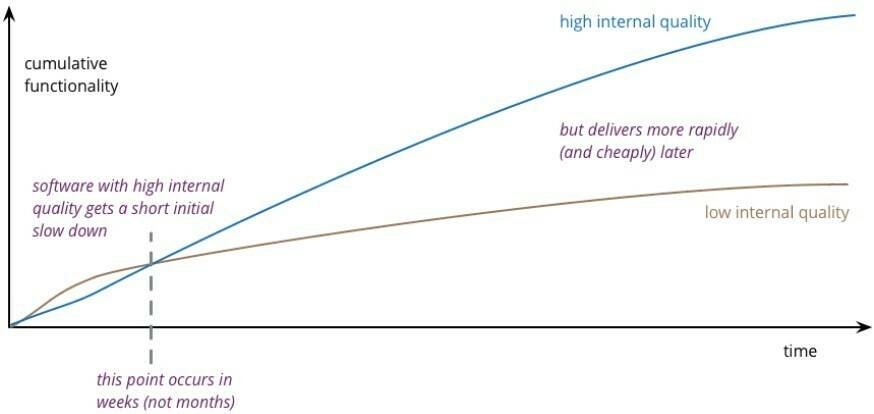
\includegraphics[width=1\textwidth]{res/quality_code.jpg}
   \caption{Erweiterbarkeit von Software mit geringer und hoher interner Qualität über Zeit \citep[][]{fowler2019}.}
   \label{fig:quality_code}
\end{figure}

Ansätze für Softwarearchitekturen hat es in den letzten Jahrzehnten einige gegeben. Darunter fallen die 
Hexagonale Architektur nach Alistair Cockburn (adaptiert von \citeauth{freeman2009}), 
DCI (\textit{Data, context, interaction}) nach \citeauth{reenskaug2009} und 
BCE (\textit{Boundary-Control-Entity}) nach \citeauth{jacobson1995}. 
Alle Varianten unterscheiden sich im Detail voneinander, haben aber die Separierung unterschiedlicher Systemaspekte durch Bildung von Schichten gemein. Alle verfolgen die Ziele testfähig, sowie unabhängig von Frameworks,  der Oberfläche, der Datenbank und sonstigen externen Komponenten zu sein. Die saubere Softwarearchitektur versucht, die bisherigen Konzepte in ein umsetzbares Konzept zu integrieren \citep[][202]{martin2018}. 

In \refAbbns{fig:clean_architecture} lässt sich eine übergreifende Abhängigkeitsregel erkennen, die besagt, dass Abhängigkeiten immer nach innen in Richtung hochrangiger Richtlinien erfolgen. Die inneren Kreise kennen die äußeren Schichten und deren Inhalt nicht. Der Kontrollfluss (\textit{flow of control}) kann aber die Grenze einer inneren zu einer äußere Schicht kreuzen, wenn die zugegriffenen Komponenten entsprechend aufgebaut sind \citep[vgl.][203]{martin2018}.


%The overriding rule that makes this architecture work is the Dependency Rule: \textit{Source code dependencies must point only inward, toward higher-level policies}.
%Nothing in an inner circle can know anything at all about something in an outer circle. In particular, the name of something declared in an outer circle must not be mentioned by the code in an inner circle. That includes functions, classes, variables, or any other named software entity  \citep[vgl.][203]{martin2018}.

\begin{figure}
  \centering
  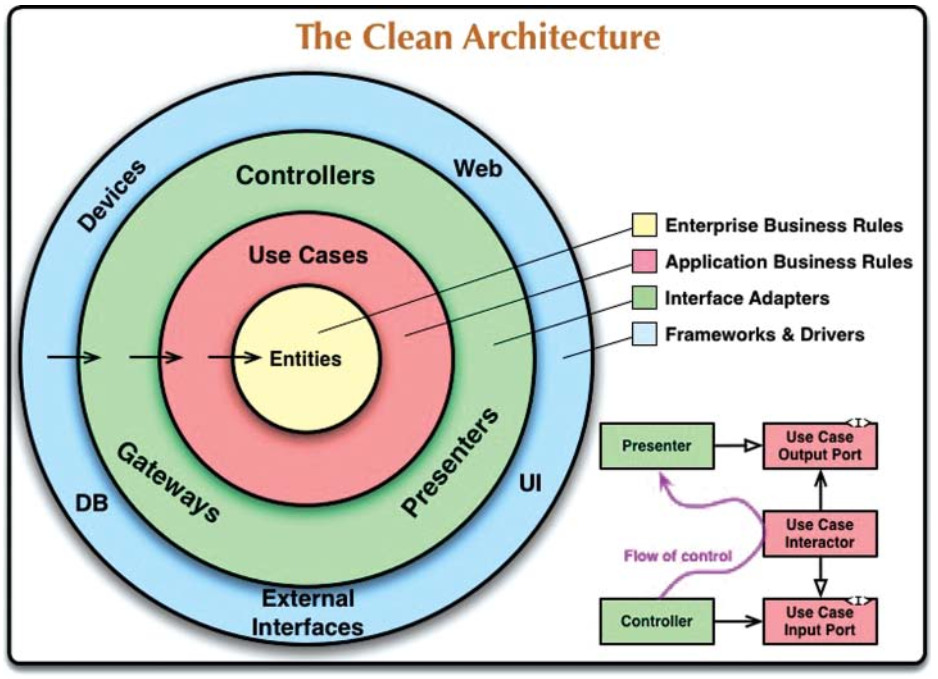
\includegraphics[width=0.9\textwidth]{res/clean_architecture.jpg}
   \caption{Schichtmodell der sauberen Softwarearchitektur \citep[][203]{martin2018}.}
   \label{fig:clean_architecture}
\end{figure}


In den nächsten Kapiteln sollen die Design"= und Komponentenprinzipien vorgestellt werden, die eine hohe interne Qualität erreichen sollen, indem sie den  Kontrollfluss und Aufbau der Schichten unterstützen. Danach wird auf Grenzlinien mit ihren Überschreitungen eingegangen, die bei der Strukturierung von Komponenten helfen können und eine höhere Modularität der Software versprechen. 


\subsection{Designprinzipien}
\label{sec:Designprinzipien}

Wartbare und erweiterbare Software beginnt mit Quellcode ohne \textit{Cruft}, ohne schlecht designten und unnötig komplizierten Quellcode. Um solchen Quellcode zu vermeiden, gibt es die Designprinzipien unter dem Akronym \textit{SOLID}. Diese und Weitere wurden in den 1980er im USENET entwickelt. Anfang 2000 wurden die fünf Prinzipien gebündelt und erhielten durch Michael Feathers ihr heutiges Acronym \citep[vgl.][58]{martin2018}.

Das Ziel ist, dass die Designprinzipien Änderungen am Quelltext zulassen, sie einfach zu verstehen sind und dass sie die Basis der Komponenten bilden. Sie sollen die Datenstrukturen und Funktionen miteinander verbinden und finden Anwendung in der mittelschichtigen Modulentwicklung \citep[vgl.][58]{martin2018}.

%\textquote[{\cite[][58]{martin2018}}]{The SOLID principles tell us how to arrange our functions and data structures into classes, and how those classes should be interconnected. The use of the word “class” does not imply that these principles are applicable only to object-oriented software. A class is simply a coupled grouping of functions and data. Every software system has such groupings, whether they are called classes or not. The SOLID principles apply to those groupings. The goal of the principles is the creation of mid-level software structures that:
%• Tolerate change,
%• Are easy to understand, and
%• Are the basis of components that can be used in many software systems. 
%The term “mid-level” refers to the fact that these principles are applied by programmers working at the module level. They are applied just above the level of the code and help to define the kinds of software structures used within modules and components.
%The history of the SOLID principles is long. I began to assemble them in the late 1980s while debating software design principles with others on USENET (an early kind of Facebook). Over the years, the principles have shifted and changed. Some were deleted. Others were merged. Still others were added. The final grouping stabilized in the early 2000s, although I presented them in a different order. In 2004 or thereabouts, Michael Feathers sent me an email saying that if I rearranged the principles, their first words would spell the word SOLID—and thus the SOLID principles were born.}

Das Akronym \textit{SOLID} besteht aus folgenden Designprinzipien:

\begin{itemize}
\item SRP: Single Responsibility Principle
\item OCP: Open-Closed Principle
\item LSP: Liskov Substitution Principle
\item ISP: Interface Segregation Principle
\item DIP: Dependency Inversion Principle
\end{itemize}

Sie werden in den folgenden Kapiteln kurz beschreiben und erläutert.

%\textquote[{\cite[][59]{martin2018}}]{
%SRP: The Single Responsibility Principle
%An active corollary to Conway’s law: The best structure for a software system is heavily influenced by the social structure of the organization that uses it so that each software module has one, and only one, reason to change.
%• OCP: The Open-Closed Principle
%Bertrand Meyer made this principle famous in the 1980s. The gist is that for software systems to be easy to change, they must be designed to allow the behavior of those systems to be changed by adding new code, rather than changing existing code.
%• LSP: The Liskov Substitution Principle
%Barbara Liskov’s famous definition of subtypes, from 1988. In short, this principle says that to build software systems from interchangeable parts, those parts must adhere to a contract that allows those parts to be substituted one for another.
%• ISP: The Interface Segregation Principle
%This principle advises software designers to avoid depending on things that they don’t use. 
%• DIP: The Dependency Inversion Principle
%The code that implements high-level policy should not depend on the code that implements low-level details. Rather, details should depend on policies.}


%SOLID -> besteht aus den unten gelisteten, auf L und I wird verichtet, da sie für eine Restrukturierung der Transaktionserfassung nicht benötigt wird.

%Was hat \citep{Noback2018} dazu gesagt?


\subsubsection{SRP: Single Responsibility Principle}

Das \ac{SRP} geht auf das Gesetz von Conway zurück, was besagt: 
\textquote[{\cite[][31]{conway1968}}]{[...] organizations which design systems [...] are constrained to produce designs which are copies of the communication structures of these organizations.}. Das bedeutet, dass die logische Struktur von Software sich an der Organisation und deren Struktur und Sprachgebrauch orientiert und sie kopiert.

Das \ac{SRP} besagt, dass es nur einen Grund geben sollte ein Modul zu ändern. Dieses Modul sollte nur für einen einzigen Akteur verantwortlich sein. Unter Modul kann hier eine Datei verstanden werden (im Java Umfeld wäre dies \zb eine Klasse), unter der ein Satz kohärenter Funktionen und Datenstrukturen gesammelt wird \citep[][62]{martin2018}. 

Ein Beispiel für einen Verstoß gegen das \ac{SRP} kann anhand folgendem Beispiel veranschaulicht werden: \refAbbns{fig:srp_false} zeigt eine Klasse, die eine DVD repräsentiert. Eine DVD enthält Informationen über den Titel des Films und wann dieser veröffentlicht worden ist (\code{getDetails()}). Zudem kann eine DVD gespeichert werden (\code{save()}). Es gibt zwei Akteure, die Interesse an der DVD haben. Einerseits der \textit{Cineast}, der Informationen über die DVD erhalten möchte, und andererseits der \textit{Admin}, der neue Filme erstellt oder an bestehenden Filmen fehlerhafte Daten korrigiert und diese speichert. Ergeben sich zeitgleich Änderungen an der Speicherung und den bereitgestellten Informationen, kann es zu Konflikten beim zusammenführen kommen. Das Modul \textit{DVD} hat in diesem Beispiel nicht die Verantwortlichkeit gegenüber einem einzigen Akteur.

\begin{figure}
  \centering
  \includegraphics[width=.4\textwidth]{build/generated-uml/srp_false.png}
   \caption{Das Modul \textit{DVD} wird von zwei Akteuren verwendet.}
   \label{fig:srp_false}
\end{figure}

Das Problem kann gelöst werden, indem die Verantwortlichkeit gegenüber einem Akteur in verschiedene Module aufgeteilt wird (\refAbb{fig:srp_okay}). Die Module können getrennt voneinander weiterentwickelt werden.

\begin{figure}
  \centering
  \includegraphics[width=.7\textwidth]{build/generated-uml/srp_okay.png}
   \caption{Das Modul \textit{DVD} wird aufgeteilt. Die Details verbleiben in dem ursprünglichen Modul. Es wird ein eigenes Modul für die Speicherung einer \textit{DVD} erzeugt.}
   \label{fig:srp_okay}
\end{figure}


\subsubsection{OCP: Open-Closed Principle}

\textquote[{\cite[][57]{meyer1997}}]{Modules should be both open and closed.}. Mit dieser Formulierung wollte \citeauth{meyer1997} ausdrücken, dass ein Modul offen für Erweiterungen sein soll, aber geschlossen für Änderungen. Ein Modul, welches von anderen Modulen verwendet wird, soll nicht selbst geändert werden. Eher soll ein neues Modul erstellt werden, das vom alten Modul erbt und bestimmte Methoden oder Datenstrukturen ersetzt. \citeauth{meyer1997} weist aber darauf hin, dass dies eine Vorgehensweise für Module ist, die außerhalb des eigenen Zugriffsbereichs liegen. Wenn es sich um Fehler in eigenen Modulen handelt, dürfen und müssen diese entsprechend korrigiert werden \citep[vgl.][60\psq]{meyer1997}. 

\begin{figure}
  \centering
  \includegraphics[width=.6\textwidth]{build/generated-uml/ocp_step_one.png}
   \caption{Ausgangssituation vom Druck einer PDF.}
   \label{fig:ocp_step_one}
\end{figure}

\begin{figure}
  \centering
  \includegraphics[width=.8\textwidth]{build/generated-uml/ocp_step_two.png}
   \caption{Aufteilung in Komponenten und Module.}
   \label{fig:ocp_step_two}
\end{figure}

\citeauth{martin2018} beschreibt das \ac{OCP} in ähnlicher Weise, geht aber noch einen Schritt weiter. Er verbindet das Prinzip mit dem \ac{DIP}. Die Kombination aus beiden Prinzipien erhält eine größere Signifikanz auf der Ebene architektonischer Komponenten \citep[vgl.][70]{martin2018}. In \refAbbns{fig:ocp_step_one} ist eine Struktur aufgebaut, die einen Export einer Filmdatenbank darstellt. Wenn diese um einen CSV Export erweitert werden soll, könnte einfach eine weitere Klasse erstellt werden, die den \code{MovieCollector} verwendet, um die Daten für die CSV Datei zu ermitteln. Das funktioniert bis sich der \code{MovieCollector} ändert. Ab diesen Zeitpunkt müssen drei Module angefasst werden: \code{MovieCollector}, \code{PdfExporter} und das neue Modul \code{CsvExporter}.

Die Architektur sollte so gestaltet werden, dass Änderungen nur an einer Stelle erfolgen müssen und andere Module und Komponenten davon nicht betroffen sind. Eine Methode wäre, die Beziehungen umzudrehen und wie in \refAbbns{fig:ocp_step_two} in sich geschlossene Komponenten zu bilden (eine Komponente wird hier als UML Package dargestellt). Die \textit{Interfaces} bilden den Vertrag, den Module erfüllen müssen, um vom Modul verwendet werden zu können. Das \textit{Interface} \code{Exporter} gibt \zb an, wie der \code{Controller} die ermittelten Daten weitergeben muss um entweder ein CSV oder ein PDF zu erhalten. Beide Implementierungen müssen die Schnittstelle einhalten.

Ein weiterer Vorteil dieser Aufteilung liegt in der Modularität. Eine Komponente kann schnell ausgetauscht werden. Wenn die Datenbank gegen eine andere ausgetauscht wird oder die Filmdaten in einer Datei gespeichert werden sollen, kann diese Komponente gewechselt werden. Die neue Komponente muss nur das \textit{Interface} \code{Repository} implementieren.

\ac{OCP} hat das Ziel ein System so zu gestalten, dass Erweiterungen leicht eingearbeitet werden können und Modifikationen keinen hohen Einfluss auf andere Komponenten und Module haben. Komponenten auf höheren Ebenen sollen vor Änderungen von Komponenten auf niedrigeren Ebenen geschützt werden \citep[vgl.][75]{martin2018}


\subsubsection{LSP: Liskov Substitution Principle}

Das \ac{LSP} geht auf folgender Definition zurück: \textquote[{\cite[][25]{liskov1987}}]{If for each object $o_1$ of type $S$ there is an object $o_2$ of type $T$ such that for all programs $P$ defined in terms of $T$, the behavior of $P$ is unchanged when $o_1$ is substituted for $o_2$, then $S$ is a subtype of $T$.}

In \refAbbns{fig:lsp_rec_square} ist ein Verstoß gegen die Substituierbarkeit  gegeben, da das Modul \code{User} seinen Quellcode ändern müsste, wenn es anstelle eines \code{Rectangle} ein \code{Square} verwendet wollte. Eine Möglichkeit, den Verstoß zu verhindern, wäre eine Erweiterung vom Modul \code{User}. Dieses Modul müsste \zb bei der Eingabe der Daten und der Berechnung der Fläche prüfen, ob es sich bei der Instanz um ein \code{Rectangle} oder \code{Square} handelt \citep[vgl.][79]{martin2018}.

\begin{figure}
  \centering
  \includegraphics[width=.3\textwidth]{build/generated-uml/lsp_rec_square.png}
   \caption{Problem der Substituierbarkeit von Rechteck zu Quadrat \citep[vgl.][79]{martin2018}.}
   \label{fig:lsp_rec_square}
\end{figure}

\ac{LSP} sollte bei der Gestaltung und Ausarbeitung der Softwarearchitektur beachtet werden. Ein simpler Verstoß kann die Anzahl zusätzlichen Mechanismen, wie \zb der Instanzprüfung, erhöhen \citep[vgl.][82]{martin2018}.

\subsubsection{ISP: Interface Segregation Principle}

Um Abhängigkeiten von nicht genutzten Modulen zu vermeiden, wird das \ac{ISP} verwendet. In \refAbbns{fig:isp_false} verwenden verschiedene Benutzer unterschiedliche Methoden aus einem Modul \code{OPS}. Dadurch werden alle Benutzer voneinander abhängig. Wenn eine Änderung an \code{OPS} durchgeführt wird, müssen die verschiedenen Benutzer auch neu kompiliert werden.

Dieses Problem kann vermieden werden, wenn die Operationen in einzelne Interfaces aufgeteilt werden (\refAbb{fig:isp_okay}). In diesem Fall wäre \code{User1} nur noch von \code{U1Ops} abhängig, aber nicht mehr zu \code{OPS} \citep[vgl.][85]{martin2018}.

\begin{figure}
  \centering
  \includegraphics[width=.4\textwidth]{build/generated-uml/isp_false.png}
   \caption{\code{User1} verwendet \code{OPS} und stellt damit eine indirekte Abhängigkeit zu \code{User2} und \code{User3} her \citep[vgl.][84]{martin2018}.}
   \label{fig:isp_false}
\end{figure}

\begin{figure}
  \centering
  \includegraphics[width=.4\textwidth]{build/generated-uml/isp_okay.png}
   \caption{Jeder Benutzer erhält eine Schnittstelle für seine Operation. \code{User1} ist nur noch von \code{U1Ops} abhängig, aber nicht mehr von \code{OPS} \citep[vgl.][85]{martin2018}.}
   \label{fig:isp_okay}
\end{figure}

Dieses Prinzip kann auch bei Abhängigkeiten zu anderen Bibliotheken bedacht werden. Wenn ein System ein Framework nutzt, das eine bestimmte Datenbank  verwendet, kann folgendes passieren: Mit der Aktualisierung der Datenbank muss auch das Framework und \ggf in Abhängigkeit dazu das System selbst aktualisiert werden. Bei einer losen Kopplung nach \ac{ISP} wäre dies nicht der Fall \citep[vgl.][86]{martin2018}.

\subsubsection{DIP: Dependency Inversion Principle}

Das \ac{DIP} besagt, dass flexible Systeme nur auf Abstraktionen aber nicht auf Konkretionen verweisen sollen. Dies lässt sich nicht immer vermeiden und sollte daher nicht erzwungen werden. Hier muss in Betracht gezogen werden, ob ein Modul in sich stabil ist und selten bis gar nicht geändert wird (\zb in Java die Klasse \code{java.lang.String}). Abhängigkeiten zu volatilen Konkretionen hingegen sollten über eine stabile Abstraktion erfolgen.
In Hinblick darauf lassen sich bestimmte Programmierpraktiken herleiten:
\begin{itemize}
\item Es sollen keine konkreten Module referenziert werden. 
\item Es soll nicht von konkreten Modulen geerbt werden.
\item Es sollen keine konkreten Methoden abstrakter Module überschrieben werden.
\item Es sollen keine Namen von konkreten Modulen genannt werden.
\end{itemize}
Um unerwünschte Abhängigkeiten zu vermeiden, kann \zb das Design Pattern \textit{Abstract Factory} (\refAbb{fig:dip_factory}) betrachtet werden \citep[vgl.][87\psq]{martin2018}. 

Die Aufteilung in \code{App} und \code{Comp} solle hier zwei verschiedene Komponenten darstellen. Das Klasse \code{Application} hat nur Schnittstellen in Abhängigkeit. Die Implementierungen befinden sich in einer anderen Komponente. Der einzige Verstoß gegen das \ac{DIP} ist der Verweis von \code{FactoryImpl} auf \code{ConcreteImpl}. Dieser lässt sich aber nicht vermeiden.

\begin{figure}
  \centering
  \includegraphics[width=.6\textwidth]{build/generated-uml/dip_factory.png}
   \caption{Angewandtes Design Pattern \textit{Abstract Factory} \citep[vgl.][90]{martin2018}.}
   \label{fig:dip_factory}
\end{figure}

Abhängigkeiten können auch dann entstehen, wenn eine Anwendung \bspw eine Laufzeitumgebung benötigt, wie \zb ein \ac{JRE}. Bei der Auslieferung der Software muss darauf geachtet werden, dass auf dem Zielsystem \ggf kein \ac{JRE} installiert ist, oder es in einer falschen Version zur Verfügung steht. Dies sind grundsätzlich Risiken, die abgewägt werden müssen \citep[vgl.][]{schuchert2013}. 

\ac{DIP} kann mit zwei weiteren Prinzipien kombiniert werden: \ac{DI} und \ac{IoC}. \ac{DI} bestimmt, wie Abhängigkeiten aufgelöst werden. Am Beispiel von einem Brettspiel: Der Spieler nimmt nicht die Würfel und rollt diese in seinem Zug, sondern das Spiel gibt dem Spieler die Würfel, wenn er am Zug ist. Mit welchen Würfeln gespielt wird, entscheidet das Spiel. Bei \ac{IoC} wird gesteuert, wer eine Nachricht initiiert. Ruft der Quellcode eine Methode aus dem Framework auf, oder ruft das Framework zurück? Wenn eine Anwendung auf das Framework zugreift, handelt es sich nicht um \ac{IoC}. Wenn ein Framework aber Quellcode der Anwendung aufruft, schon. Dies geht auf \textit{Hollywood's Law} zurück: \textquote[{\cite[][218]{sweet1985}}]{Don‘t call us, we’ll call you.}. Bei einem Brettspiel würde das Spiel die Interaktionen der Spieler orchestrieren und dessen Aktionen anfordern \citep[vgl.][]{schuchert2013}.

Die Kombination dieser drei Prinzipien bietet viele Vorteile zur Strukturierung von Quellcode und der Vermeidung von ungewollten Abhängigkeiten. \ac{DIP} stellt hierfür die Struktur dar, während \ac{DI} für die Versorgung konkreter Module sorgt. Über \ac{IoC} kann eine Abhängigkeit durch \textit{Hollywood's Law} umgedreht werden.

%In 2004, Martin Fowler published an article on Dependency Injection (DI) and Inversion of Control (IoC) . Is the DIP the same as DI, or IoC? No, but they play nice together. When Robert Martin first discussed the DIP, he equated it a first-class combination of the Open Closed Principle and the and the Liskov Substitution Principle, important enough to warrant its own name. Here's a synopsis of all three terms using some examples: \citep[vgl.][]{schuchert2013}

%DI is about how one object acquires a dependency. When a dependency is provided externally, then the system is using DI. IoC is about who initiates the call. If your code initiates a call, it is not IoC, if the container/system/library calls back into code that you provided it, is it IoC. \citep[vgl.][]{schuchert2013}

%DIP, on the other hand, is about the level of the abstraction in the messages sent from your code to the thing it is calling. To be sure, using DI or IoC with DIP tends to be more expressive, powerful and domain-aligned, but they are about different dimensions, or forces, in an overall problem. DI is about wiring, IoC is about direction, and DIP is about shape. \citep[vgl.][]{schuchert2013}


\subsection{Komponentenprinzipien}
\label{sec:Komponentenprinzipien}

Komponenten sind die kleinsten veröffentlichbaren Einheiten eines Systems. In Java können sie als \code{.jar} Dateien in das System mit eingebunden werden. Komponenten können aber auch programmatisch in einem System eingebracht werden. Eine Komponente besitzt die Fähigkeit unabhängig von anderen Komponenten entwickelt zu werden \citep[vgl.][96]{martin2018}.

Komponenten weisen die Eigenschaft der Kohäsion und der Kopplung auf. Dabei existiert die Köhasion innerhalb einer Komponente und die Kopplung zwischen verschiedenen Komponenten \citep[vgl.][131]{voorhees2020}.

%Note the contrast between coupling and cohesion—coupling exists between two modules while cohesion exists within one module \citep[vgl.][131]{voorhees2020}.

Im Folgenden werden Prinzipien der Komponentenkohäsion und der "=kopplung vorgestellt. Dabei wird bei der Komponentenkopplung auf zwei Metriken (\textit{positional stability} und \textit{abstractness} einer Komponente) eingegangen, anhand deren man die Kopplung einzelner Komponenten untereinander bemessen kann.

\subsubsection{Komponentenkohäsion}

Das Ausmaß, wie Module innerhalb einer Komponente zusammenhängen, nennt sich Kohäsion. Eine hohe Kohäsion ist ein Merkmal gut entworfener Komponenten in einem System. Wenn Komponenten für Module verantwortlich sind, die nicht miteinander zusammenhängen, wurde die Funktionalität schlecht verteilt \citep[vgl.][797]{gui2009}.

%Cohesion is the extent to which the functions performed by a subsystem are related. If a subcomponent is responsible for a number of unrelated functions then the functionality has been poorly distributed to subcomponents. Hence high cohesion is a characteristic of a well designed subcomponent \citep[vgl.][797]{gui2009}.

Eine hohe Kohäsion ist auch daran zu erkennen, dass eine Komponente mit einer einzigen Aufgabe schwer in weitere Komponenten aufzuteilen ist und dass sich einzelne Module aus der Komponente nicht trennen lassen. Eine Komponente hingegen, deren Aufgabenbereich zu weit gefasst ist und zu viele Abhängigkeiten aufweist, kann folgende Probleme aufweisen: Sie ist schwer zu verstehen, wiederzuverwenden, zu pflegen und ständigen Änderungen ausgesetzt \citep[vgl.][131]{voorhees2020}.

%Having a module with one basic purpose that is hard to split into separate units is called high cohesion or strong cohesion. A good design is one that exhibits highly cohesive modules. Having a module that contains many basic purposes (i.e., many responsibilities) is called low cohesion or weak cohesion. A bad design is one that exhibits low cohesive modules.
%A class with low cohesion does many unrelated things or does too much work. Such classes are undesirable; they suffer from the following problems:
%• Hard to comprehend
%• Hard to reuse
%• Hard to maintain
%• Delicate; constantly affected by change \citep[vgl.][131]{voorhees2020}.

Zum Zusammenfassen von Komponenten gibt \citeauth{martin2018} drei Prinzipien vor:
\begin{itemize}
\item \ac{REP}
\item \ac{CCP}
\item \ac{CRP}
\end{itemize}

Softwarekomponenten, die wiederverwendet werden sollen, müssen für das \ac{REP} erst einem Releaseprozess unterlaufen und eine Versionsnummer erhalten \citep[vgl.][104]{martin2018}. Das bedeutet gleichzeitig, dass Module nicht einfach zu einer Komponente zusammengeworfen werden, sondern einer übergreifenden Aufgabe dienen sollen \citep[vgl.][105]{martin2018}.

%The Reuse/Release Equivalence Principle (REP) is a principle that seems obvious, at least in hindsight. People who want to reuse software components cannot, and will not, do so unless those components are tracked through a release process and are given release numbers \citep[vgl.][104]{martin2018}.

%From a software design and architecture point of view, this principle means that the classes and modules that are formed into a component must belong to a cohesive group. The component cannot simply consist of a random hodgepodge of classes and modules; instead, there must be some overarching theme or purpose that those modules all share \citep[vgl.][105]{martin2018}.

Beim \ac{CCP} wird verlangt, Module, die zur selben Zeit und aus demselben Grund geändert werden, in eine Komponente zu fassen. Wenn Module diese Eigenschaft nicht aufweisen, sollten sie in verschiedene Komponenten gegliedert werden \citep[vgl.][105]{martin2018}.
 
%Gather into components those classes that change for the same reasons and at the same times. Separate into different components those classes that change at different times and for different reasons \citep[vgl.][105]{martin2018}. 

%MAYBE: For most applications, maintainability is more important than reusability. If the code in an application must change, you would rather that all of the changes occur in one component, rather than being distributed across many components. If changes are confined to a single component, then we need to redeploy only the one changed component. Other components that don’t depend on the changed component do not need to be revalidated or redeployed \citep[vgl.][106]{martin2018}.

Das \ac{CRP} besagt, dass gemeinsam genutzte Komponenten in eine Komponente übergehen sollen, sofern sie immer miteinander verwendet werden. So werden unnötige Abhängkeiten vermieden \citep[vgl.][107]{martin2018}.

%Don’t force users of a component to depend on things they don’t need. It states that classes and modules that tend to be reused together belong in the same component \citep[vgl.][107]{martin2018}. 

%Therefore the CRP tells us more about which classes shouldn’t be together than about which classes should be together. The CRP says that classes that are not tightly bound to each other should not be in the same component \citep[vgl.][108]{martin2018}.
 

\subsubsection{Komponentenkopplung}

Kopplung ist die Interaktion von Komponenten untereinander. Wenn die Kopplung zwischen Komponenten stärker ist, kann eine Änderung an einer Komponente auch Änderungen an den abhängigen nach sich ziehen. Eine lose Kopplung ist daher eine gewünschte Eigenschaft \citep[vgl.][797]{gui2009}.

%Coupling is the extent to which the various subcomponents interact. If  hey are highly interdependent then changes to one are likely to have  significant effects on the behavior of others. Hence loose coupling  between its subcomponents is a desirable characteristic of a component \citep[vgl.][797]{gui2009}.

Umso weniger Verbindungen zwischen Komponenten bestehen, desto weniger Aufwand entsteht in der Wartung, Reparatur oder im Test einer Komponente. Ein gutes Design weist daher eine geringe Kopplung auf. Eine starke Kopplung hingegen bedeutet: Änderungen von Abhängigkeiten müssen in lokale Komponenten eingepflegt werden, eine Komponente ist isoliert schwieriger zu verstehen und die Wiederverwendung wird durch benötigte Abhängigkeiten schwieriger \citep[vgl.][130]{voorhees2020}.

%The coupling definitions indicate that coupling describes the amount of connectedness between two or more modules. Thus, a design that has only one module cannot exhibit coupling. That is, coupling can only be described between distinct modules. Our intuition suggests having fewer connections between modules mean there is less to test, maintain, and fix. Having fewer connections between modules is called low coupling, loose coupling, or weak coupling. A good design is one that exhibits low coupling between its modules. In contrast, more connections between modules means there is more to test, maintain, and fix. Having more connections between modules is called high coupling, tight coupling, or strong coupling. A bad design is one that exhibits high coupling between its modules  \citep[vgl.][130]{voorhees2020}.

%A class with high (or strong) coupling relies on many other classes. Such classes may be undesirable; some suffer from the following problems:
%• Changes in related classes force local changes
%• Harder to understand in isolation
%• Harder to reuse because its use requires the additional presence of the classes on which it is dependent   \citep[vgl.][130]{voorhees2020}.


Um Komponenten miteinander zu verbinden, gibt \citeauth{martin2018} drei verschiedene Prinzipien vor:
\begin{itemize}
\item \ac{ADP}
\item \ac{SDP}
\item \ac{SAP}
\end{itemize}

Das \ac{ADP} besagt, dass keine zyklischen Abhängigkeiten zwischen Komponenten erlaubt werden und es sich um einen \ac{DAG} handeln soll. Bei einem \ac{DAG} kann von einer beliebigen Stelle einem Pfad gefolgt werden, ohne wieder am Ausgangspunkt anzugelagen \citep[vgl.][114]{martin2018}. 

In \refAbbns{fig:adp_false} ist dies nicht der Fall. Das Problem kann aber auf zwei Arten behoben werden. Zum einen kann eine dritte Komponente mit entsprechenden Schnittstellen gebildet werden und beide Komponenten zeigen auf diese  (\refAbb{fig:adp_okay}). Die andere Variante ist die Anwendung vom \ac{DIP}. Hierdurch wird eine Schnittstelle in eine Komponente aufgenommen, wodurch sich die Beziehung umdreht (\refAbb{fig:adp_okay_2}).

\begin{figure}
  \centering
  \includegraphics[height=1.2cm]{build/generated-uml/adp_false.png}
   \caption{Zyklische Abhängigkeit zwischen zwei Komponenten.}
   \label{fig:adp_false}
\end{figure}

\begin{figure}
  \centering
  \includegraphics[height=1.2cm]{build/generated-uml/adp_okay.png}
   \caption{Auflösung der zyklischen Abhängigkeit durch eine dritte Komponente.}
   \label{fig:adp_okay}
\end{figure}

\begin{figure}
  \centering
  \includegraphics[width=5cm]{build/generated-uml/adp_okay_2.png}
   \caption{Auflösung der zyklischen Abhängigkeit durch Anwendung von \ac{DIP}. Die Verbindung von \code{A} nach \code{B} wird aufgelöst und umgekehrt. Die Beziehung besteht nur noch logisch (gestrichelter Pfeil). }
   \label{fig:adp_okay_2}
\end{figure}


%Allow no cycles in the component dependency graph \citep[vgl.][112]{martin2018}.

%Regardless of which component you begin at, it is impossible to follow the dependency relationships and wind up back at that component. This structure has no cycles. It is a directed acyclic graph (DAG) \citep[vgl.][114]{martin2018}. 

%It is always possible to break a cycle of components and reinstate the dependency graph as a DAG. There are two primary mechanisms for doing so ... \citep[vgl.][117]{martin2018}.
 
Das \ac{SDP} besagt, dass eine Komponente nur auf eine anderen Komponente verweisen soll, wenn diese stabiler ist. Dabei misst sich die \textit{positional stability} (im Folgenden Instabilität) anhand der Formel
\begin{equation}
I = F_o / (F_i + F_o).
\end{equation}
$F_i$ sind dabei die eingehenden Abhängigkeiten der Komponente. Hier werden alle Module gezählt, die auf die Komponente zugreifen. $F_o$ sind alle ausgehenden Abhängigkeiten, bei denen die Module gezählt werden, die außerhalb verwendet werden. $I$ ist die Instabilität und nimmt einen Wert zwischen $0$ und $1$ an. Bei einem Wert von $1$ gilt die Komponente als instabil, da sie von keiner anderen Komponente verwendet wird, aber selbst sehr viele andere Komponenten verwendet. Bei $0$ besitzt eine Komponente keine Abhängigkeiten, aber wird von anderen verwendet \citep[vgl.][122]{martin2018}.
 
%Depend in the direction of stability. 

%• Fan-in: Incoming dependencies. This metric identifies the number of classes outside this component that depend on classes within the component.
%• Fan-out: Outgoing depenencies. This metric identifies the number of classes inside this component that depend on classes outside the component.
%• I: Instability: I = Fan-out , (Fan-in + Fan-out). This metric has the range [0, 1]. I = 0 indicates a maximally stable component. I = 1 indicates a maximally unstable component \citep[vgl.][122]{martin2018}
  
\ac{SAP} besagt, eine Komponente sollte so abstrakt wie stabil sein \citep[vgl.][126]{martin2018}. Dadurch verlaufen Abhängigkeiten in Richtung der Abstraktion, wodurch automatisch instabile Komponenten auf stabile Komponenten verweisen. 

Der Grad $A$ der \textit{abstractness} lässt sich über 
\begin{equation}
A = N_a/N_c
\end{equation}
berechnen. Dabei ist $N_a$ die Anzahl aller abstrakten Module, $N_c$ ist die Anzahl aller Module. $A$ liegt im Bereich zwischen $0$ und $1$. Eine Komponente mit dem Wert $0$ ist dabei komplett konkret, da keine Schnittstellen in der Komponente vorhanden sind. Bei einem Grad von $1$ gibt es keine Implementierungsdetails, sondern alle Module sind Schnittstellen \citep[vgl.][127]{martin2018}.

%A component should be as abstract as it is stable  \citep[vgl.][126]{martin2018}.

%• Nc: The number of classes in the component.
%• Na: The number of abstract classes and interfaces in the component.
%• A: Abstractness. A = Na , Nc.
%The A metric ranges from 0 to 1. A value of 0 implies that the component has no abstract classes at all. A value of 1 implies that the component contains nothing but abstract classes  \citep[vgl.][127]{martin2018}.

Wenn beide Werte zusammengenommen werden, kann eine Komponente auf einem Graph, wie in \refAbbns{fig:i_a_graph}, verortet werden. Die Komponenten befinden sich idealerweise auf oder in der Nähe der Hauptreihe (\textit{Main Sequence}). Komponenten in der \textit{Zone of Pain} und der \textit{Zone of Uselessness} sollten vermieden werden. Solche Komponenten lassen sich schwer aktualisieren \bzw erfüllen schlicht keinen Zweck und sind damit nutzlos \citep[vgl.][128\psqq]{martin2018}. Die Distanz $D$ zu Hauptreihe berechnet sich mit 
\begin{equation}
D = |A + I -1|
\end{equation}
\citep[vgl.][130]{martin2018}.

\begin{figure}
  \centering
  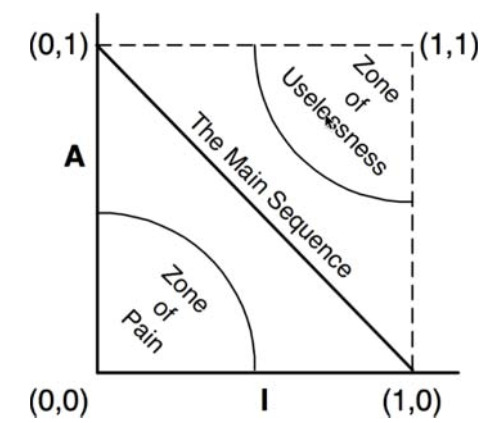
\includegraphics[width=7cm]{res/i_a_graph.jpg}
   \caption{Komponenten, deren Instabilität und Abstraktheit berechnet wurde, können in einem solchen Graphen verortet werden \citep[][128]{martin2018}.}
   \label{fig:i_a_graph}
\end{figure}


\citeauth{martin2018} trifft keine Aussage darüber, wann $D$ zu groß ist. Es wird nur gesagt, dass sich $D$ mit jeder Restrukturierung Null nähern soll.

\subsection{Grenzlinien und "=überschreitungen}
\label{sec:grenzen}

Grenzen verlaufen im Groben zwischen den Schichten, wie bereits in \refAbbns{fig:clean_architecture} schematisch dargestellt. Es wird versucht Grenzen zwischen Dingen zu ziehen, die wichtig sind oder nur Details darstellen. Die Oberfläche ist nicht abhängig von den Geschäftsregeln und für die Datenbank spielen sie ebenso keine Rolle. Dementsprechend sollte eine Grenze gezogen werden, wie \zb in \refAbbns{fig:border_gui_br_db} dargestellt \citep[vgl.][165\psq]{martin2018}. Die Oberfläche und die Datenbank sind hier ein Detail des Systems. Ob eine \textit{MySql}, \textit{Oracle} oder \textit{PostgreSQL} als Datenbank verwendet wird oder die Daten im Dateisystem gespeichert werden, ist für die Geschäftsregeln unerheblich. Es wird lediglich eine Schnittstelle angeboten, über die Daten an eine Komponente gegeben werden. Welche Komponente dies ist, kann auf einen späteren Zeitpunkt verschoben werden. Das Gleiche gilt für das \ac{GUI}. Ob nun eine REST-Schnittstelle\footnote{Representational State Transfer} oder direkt eine Benutzeroberfläche für \textit{Windows} oder eine Applikation für \textit{Android} erstellt wird, ist auch für die Geschäftsregeln nicht wichtig. Sie stehen im Kern des Systems. 

\begin{figure}
  \centering
  \includegraphics[width=.5\textwidth]{build/generated-uml/border_gui_br_db.png}
   \caption{Die Geschäftsregeln werden von den Komponenten \code{GUI} und \code{DB} verwendet. Jede Komponente ist für sich autark.}
   \label{fig:border_gui_br_db}
\end{figure}

% was wird abgegrenzt
%You draw lines between things that matter and things that don’t. The GUI doesn’t matter to the business rules, so there should be a line between them. The database doesn’t matter to the GUI, so there should be a line between them. The database doesn’t matter to the business rules, so there should be a line between them \citep[vgl.][165\psq]{martin2018}.

Ein weiterer Punkt ist, dass Grenzen dort gezogen werden, wo sich Änderungen aus unterschiedlichen Gründen ergeben \citep[vgl.][173]{martin2018}.

%Boundaries are drawn where there is an axis of change. The components on one side of the boundary change at different rates, and for different reasons, than the components on the other side of the boundary \citep[vgl.][173]{martin2018}.

% was ist Kontrollfluss?


%At the lower right of the diagram in Figure 22.1 is an example of how we cross the circle boundaries. It shows the controllers and presenters communicating with the use cases in the next layer. Note the flow of control: It begins in the controller, moves through the use case, and then winds up executing in the presenter. Note also the source code dependencies: Each points inward toward the use cases. We usually resolve this apparent contradiction by using the Dependency Inversion Principle. In a language like Java, for example, we would arrange interfaces and inheritance relationships such that the source code dependencies oppose the flow of control at just the right points across the boundary \citep[vgl.][206]{martin2018}.


Zur Laufzeit ist eine Grenzüberschreitung nur eine Funktion, die auf der anderen Seite einer Grenze eine andere Funktion über eine Schnittstelle aufruft. Hierbei muss nur darauf geachtet werden, wie die Abhängigkeiten verwaltet werden \citep[vgl.][176]{martin2018}.

%At runtime, a boundary crossing is nothing more than a function on one side of the boundary calling a function on the other side and passing along some data. The trick to creating an appropriate boundary crossing is t´o manage the source code dependencies  \citep[vgl.][176]{martin2018}.

In \refAbbns{fig:border_cross_false} wird eine Grenzüberschreitung dargestellt, die in eine falsche Richtung verläuft. Der Kontrollfluss geht hier von einer niedrigen Schicht in eine höhere Schicht. Um dies zu vermeiden, kann Polymorphie genutzt werden (\refAbb{fig:border_cross_okay}). Hier ruft die höhere Schicht die niedrigere auf. Auch zu bemerken ist, dass das Modul \code{Data} sich auf der aufgerufenen Seite befindet \citep[vgl.][178]{martin2018}.

%In Figure 18.2, the flow of control crosses the boundary from left to right as before. The high-level Client calls the f() function of the lower-level ServiceImpl through the Service interface. Note, however, that all dependencies cross the boundary from right to left toward the higher-level component. Note, also, that the definition of the data structure is on the calling side of the boundary  \citep[vgl.][177\psq]{martin2018}.

\begin{figure}
  \centering
  \includegraphics[width=.4\textwidth]{build/generated-uml/border_cross_false.png}
   \caption{Grenzüberschreitung aus einer inneren Schicht (\code{Business}) zu einer äußeren (\code{DB}).}
   \label{fig:border_cross_false}
\end{figure}

\begin{figure}
  \centering
  \includegraphics[width=.6\textwidth]{build/generated-uml/border_cross_okay.png}
   \caption{Umkehr der Abhängigkeit durch Verwendung von Schnittstellen. Die äußere Schicht (\code{DB}) verwendet die innere Schicht (\code{Business}).}
   \label{fig:border_cross_okay}
\end{figure}

Hochrangige Abhängigkeiten und Komponenten sollten als \textit{Plugin} gesehen werden. Sie werden bei Bedarf hinzugenommen, wirken sich aber nicht auf die Geschäftsregeln aus und haben auch keinerlei internes Wissen über die Geschäftsregeln \citep[vgl.][181]{martin2018}.

%Lower-level services should “plug in” to higher-level services. The source code of higher-level services must not contain any specific physical knowledge (e.g., a URI) of any lower-level service \citep[vgl.][181]{martin2018}.

Die Aufteilung in Komponenten kann teuer sein, wenn \zb in Java für jede Komponente eine eigene \code{.jar}-Datei erstellt wird. Hierfür gibt es partielle Grenzen, die auf eine Separierung in verschiedene \code{.jar}-Dateien verzichtet und die Grenzen virtuell zieht. Der Umfang des Quellcodes nimmt hierbei nicht ab \citep[vgl.][218]{martin2018}. 




